%%
%% This is file `example-1.tex',
%% generated with the docstrip utility.
%%
%% The original source files were:
%%
%% drexel-thesis.dtx  (with options: `example-part')
%% 
%% This is a generated file.
%% 
%% Copyright (C) 2010 W. Trevor King
%% 
%% This file may be distributed and/or modified under the conditions of
%% the LaTeX Project Public License, either version 1.3 of this license
%% or (at your option) any later version.  The latest version of this
%% license is in:
%% 
%%    http://www.latex-project.org/lppl.txt
%% 
%% and version 1.3 or later is part of all distributions of LaTeX version
%% 2003/06/01 or later.
%% 

\chapter{Population activity encoding }

Individual neurons in the brain are tuned to fire upon specific events such as visual stimuli of a particular type \citep{Hubel1962} .
However, even neurons that are tuned to a specific stimulus show variability in their firing rate and timing when the same stimulus is repeatedly applied \citep{Georgopoulos1982}\citep{Newsome1989}.
This indicates that individual neurons do not reliably encode sensory information, and therefore information in the brain must be represented by the firing dynamics of populations of many neurons.
This neuron population coding may take the form of variations in the average firing rate of the neurons in the population (rate coding) or variations in the synchronization between neuron spikes (temporal coding).
The temporal and rate coding may also have a functional relation, i.e. through Hebbian learning \citep{Basawaraj2019}.
Various methods of decoding the information in these population dynamics have been studied \citep{Deneve1999}\citep{Xu2019}, 
and population dynamics are incorporated into modern theories of neural computation \citep{Pitkow2017}\citep{Nadeau2020}.

Here we consider how information that is represented as population activity in one cortical area could be transferred to another cortical area via traveling waves.
For example, \citet{Heitmann2013} proposed a possible mechanism for decoding traveling waves and provided applications to the motor cortex.
Direct connections between spatially separated cortical areas are quite sparse\citep{Markov2011} as intra-cortical connectivity is mostly local in nature.
Traveling waves of neuronal activity would provide a mechanism for long-range information transfer across cortical areas 
even if there were very few direct neural connections between those areas.

To test our hypothesis of information coding and transfer we first define a population of input neurons.
These input neurons represent a neural population that is e.g. tuned to the same orientation of visual stimulus, 
so that the stimulus or other information is encoded in the firing rate of this population.
We represent the information as an average firing rate.
We simulate the population of input neurons as independent Poisson processes with the common firing rate F.
We then perform simulations of neural system to determine if the information, encoded in the firing rate of the input population,
can be transferred via traveling waves.

We have previously shown that our minicolumn model supports stimulus-evoked traveling waves across a variety of model parameters.
We now demonstrate that input from a population of neurons, simulated as Poisson spike trains, can evoke traveling waves in our quasi one-dimensional system.
The number of waves per second that travel through the minicolumn, which we term the wave arrival rate, increases as the average firing rate of the input pool of neurons is increased.
The plot of wave arrival rate versus input population firing rate resembles the activation functions of either a single neuron or a population of neurons.
This leads us to consider the SCE to have a nonlinear activation function in terms of input population rate, and to consider the SCE as encoding the input population firing rate into the wave arrival rate.

Just as a single neuron may be susceptible to noise or damage, a single SCE may also be an unreliable means of encoding and transmitting population rate information.
We therefore look at morphologies of multiple redundant SCE to enable reliable encoding and transport.
We find that simply increasing the cross-section of the SCE ...

We performed a series of computational experiments to determine how our SCE can encode and transmit population activity.
We first verified that our population of Poisson neurons can invoke traveling waves in a single SCE.
The wave rate in the single SCE was found to be proportional to the instantaneous firing rate of the population of Poisson neurons.
The relationship between population activity and wave rate resembled the activation functions of both single neurons and populations of neurons, so we termed this relationship the activation function of the SCE.
The activation function of the SCE showed significant variation across trials with randomly generated stimuli, indicating that the population rate encoding was not reliable.
We then created SCE with larger cross-section (X and Y extents) with varying topologies and observed that an ensemble of multiple SCE with loose coupling between them reduces the variation in the activation function.

\section{Population activity representation}
We wish to understand how our SCE may encode and transmit population activity.
Individual neurons in the cortex fire irregularly \citep{Maimon2009}, and the spike timing of a single neuron is generally characterized by a Poisson process with some instantaneous firing rate \citep{Gerstein1964}.
The external stimulus $I_i^{stim}$ in our simulations is generated from a population of 50 neurons that emit spikes according to independent Poisson processes characterized by a common instantaneous firing rate.
Each neuron $j$ in the input population of Poisson neurons is connected to each neuron $i$ in the bottom layer (all SCE neurons with Z=0) of the SCE with probability $P_{ij} = 1/2$.
The stimulus applied to the bottom layer is given by:
\begin{align}
 \begin{split}
  I_i(t)^{stim} &= \sum_{i,j} \sum_{t^\prime_j} S_{ij}  \Theta(t-t^\prime_j)e^{-(\frac{t-t^\prime_j}{\sigma_e})^2}\\
  S_{ij}^{excitatory} &= K^{stim} \times \mathcal{U}\{0,0.5 \} \text{ if i,j connected}\\
  S_{ij}^{inhibitory} &= K^{stim} \times \mathcal{U}\{-1,0 \} \text{ if i,j connected}\\
  S_{ij} &= 0 \text{ if i,j not connected}
 \end{split}
\end{align}
where $t^\prime_j$ are the spike times of Poisson neuron $j$, $\sigma_e=2\ ms$ is a synaptic response time constant as described above, and $K^{stim}$ is an overall connection strength weight as described above.


\section{Traveling waves are evoked by population activity}
Our first configuration is an SCE consisting of four minicolumns, each with dimensions $2x2x40$ (X/Y/Z).
The SCE parameters are $C=0.5$, $\lambda=2.5$, $\kappa=0.1$, $K^{SCE}=24$ and $K^{stim}=6$.
The other parameters are fixed for all experiments as described in Methods.

We stimulated the SCE using several instantaneous firing rates for the input population.
Traveling waves are evoked in the SCE for higher firing rates (Figure \ref{fig:sce_raster}).

\begin{figure}[!htb]
 \centering
 \caption{Poisson spike trains in the input population (bottom) evoke traveling waves in the SCE (top). 
	  Raster plots are shown for firing rates of 1 spike/second (left), 5 spikes/second (middle) and 21 spikes/second (right).  }
 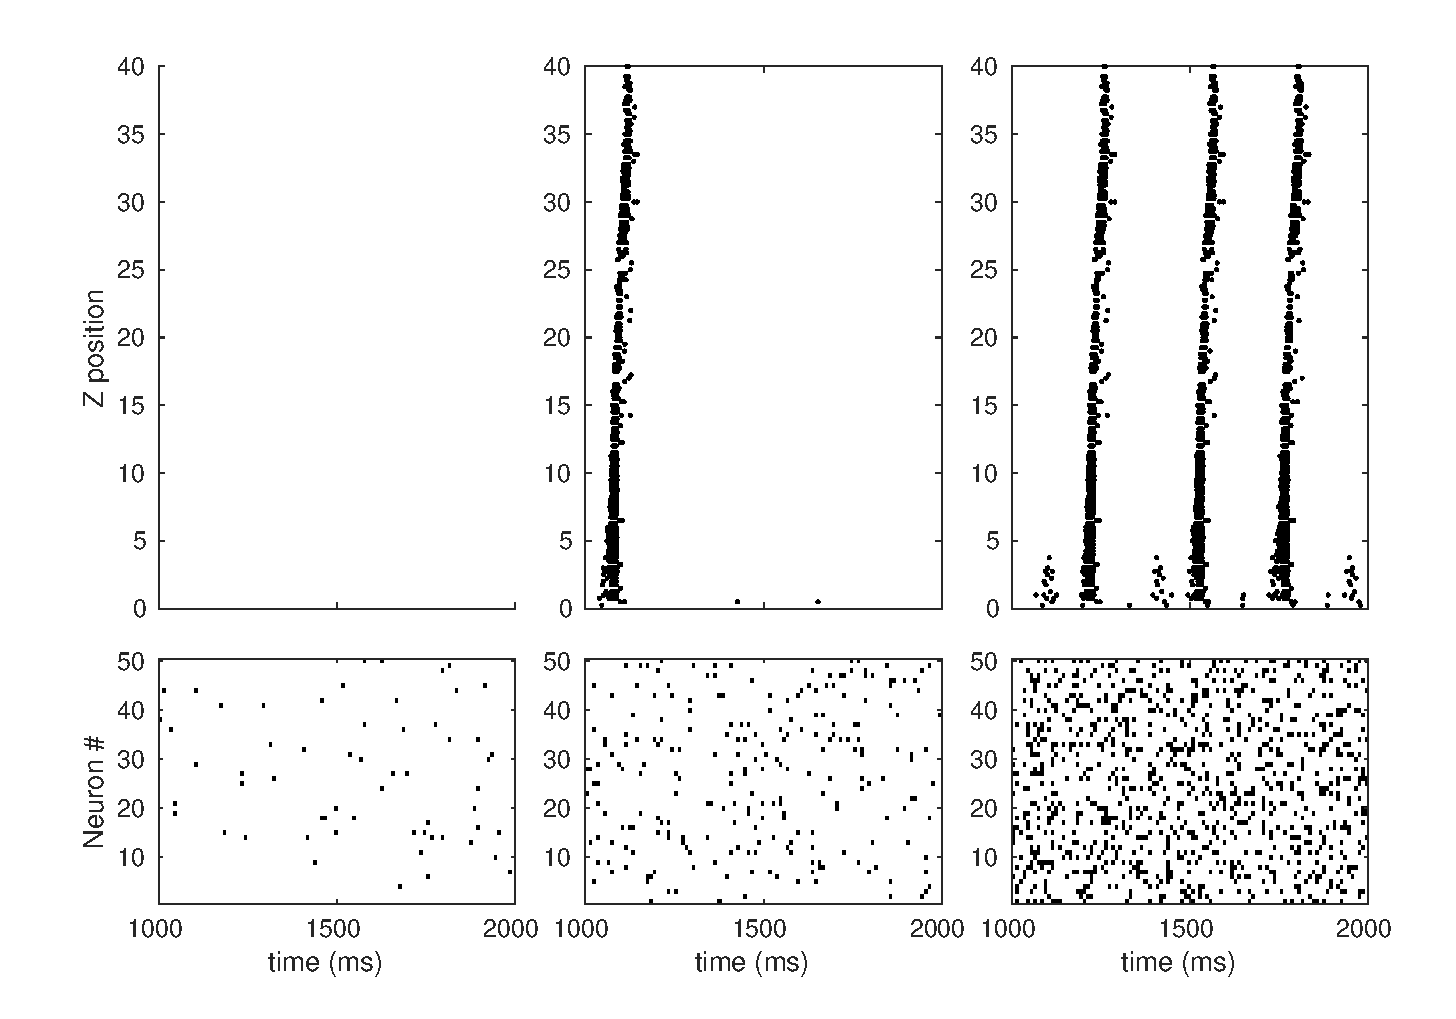
\includegraphics[width=\textwidth]{fig/SCE_2x2_FRE_rasters}
 \label{fig:sce_raster}
\end{figure}

\FloatBarrier

\section{The SCE possesses an activation function}
We stimulated the SCE with instantaneous firing rates from 1 to 21 spikes/second, with 100 random inputs created for each firing rate.
The resulting waves rates are shown in Figure \ref{fig:sce_activation_function}.
The mean wave rate showed a clear trend that is similar to a logarithmic curve. 
It also resembled the population activation rate shown in \citet{Trappenberg2010} Eq. 3.43 for the population response to slowly varying inputs:
\begin{align}
 g(x) &= \frac{1}{t^{ref}-\tau \log{(1-\frac{1}{\tau x})}}
\end{align}
where $t^{ref}$ is an absolute refractory period and $\tau$ is the charateristic response time.
We therefore consider our SCE to have an nonlinear activation function when stimulated by a  population of neurons.
This demonstrated that the SCE can be said to encode the population rate into the wave rate in a analogous manner to which single neurons and populations of neurons encode their stimulus strength into their firing rate.

\begin{figure}[!htb]
 \centering
 \caption{The SCE encodes the input population firing rate into the wave arrival rate. }
 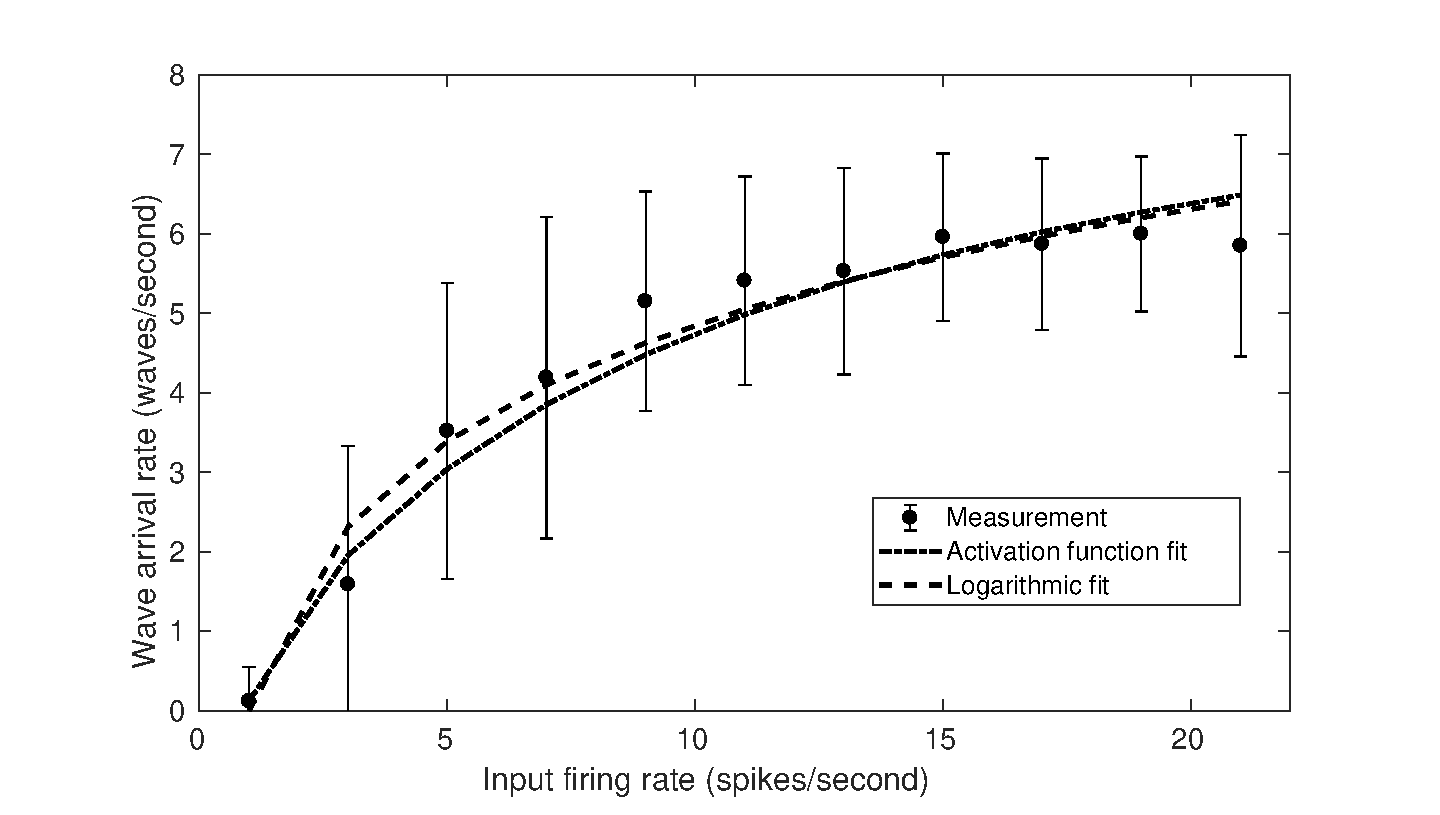
\includegraphics[width=\textwidth]{fig/SCE_2x2_FRE}
 \label{fig:sce_activation_function}
\end{figure}

Although the mean wave rates showed a clear trend, the trial-to-trial wave rates were highly variable. 
This indicates that our SCE would not reliably encode population rate into wave rate.

\FloatBarrier

\section{Adding redundant columns to the SCE can reduce variability in the activation function}
Like our SCE, individual neurons also have variable firing responses to identical stimuli.
This variability is one of the key motivations for the population activity theories of information encoding in the cortex.
We next followed a similar approach and investigated the activation function of a population of multiple redundant SCE.
Several populations of SCE were generated with different distance (and therefore connectivity), between the individual SCE.
We found that a population of four SCE, with the individual SCE separated by $2\lambda$, produced a much smoother activation function.
A population of four widely separated SCE with no connectivity between them was still highly variable.


\begin{figure}[!htb]
 \centering
 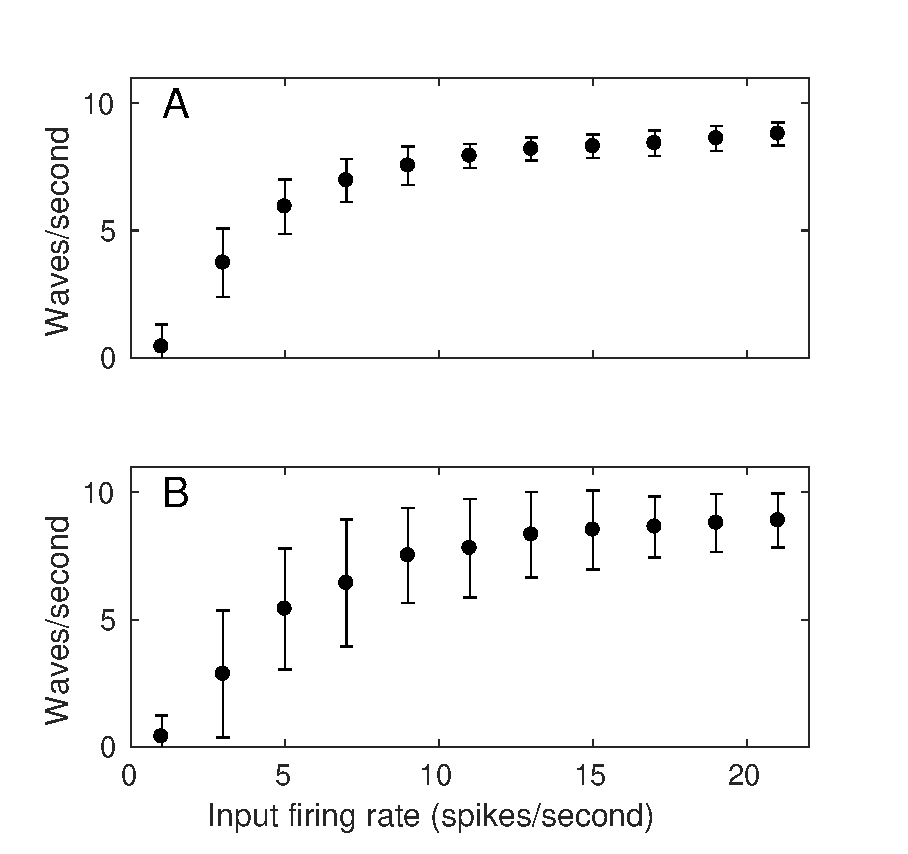
\includegraphics[width=\textwidth]{fig/OneLambdaFourLambda}
 \caption{Activation functions of a population of 4 SCEs. 
	    A: When the SCE are spaced $2\lambda$ apart the activation function shows greatly reduced variability. 
	    B: When the SCE are widely spaced with no connectivity between the SCE there is still substantial variability in the activation function.}
 \label{fig:sce_4x4_coupled_activation_function}
\end{figure}

\FloatBarrier


\endinput
%%
%% End of file `example-1.tex'.
